
%(BEGIN_QUESTION)
% Copyright 2006, Tony R. Kuphaldt, released under the Creative Commons Attribution License (v 1.0)
% This means you may do almost anything with this work of mine, so long as you give me proper credit

Et tank expert-system viser følgende trykkverdier fra sine tre transmittere:

$$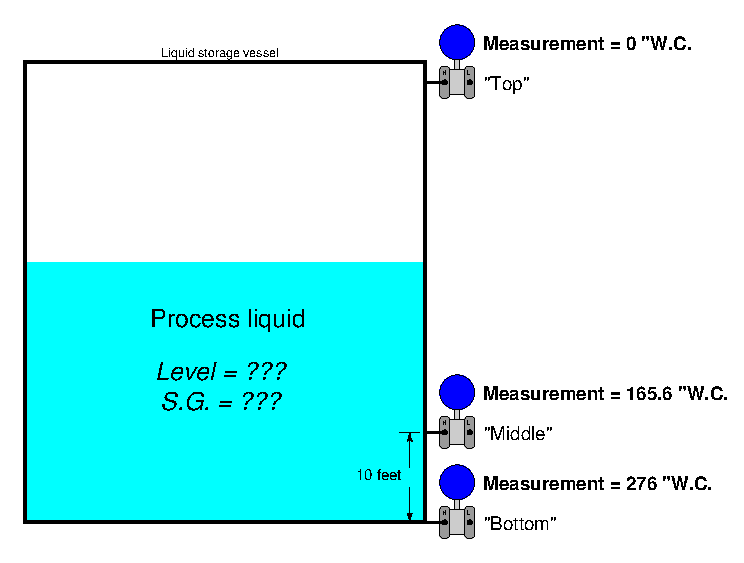
\includegraphics[width=15.5cm]{i00255x01.eps}$$

Bestem væskenivået i tanken og spesifikk vekt.  Forklar tydelig hvordan du kom frem til svarene.

\underbar{file i00255}
%(END_QUESTION)





%(BEGIN_ANSWER)

At ``Top''-transmitteren viser 0 inches water column forteller oss at tanken er ventilert, eller i det minste at det ikke er damptrykksoppbygging.  Det gjør oppgaven med å finne nivå og tetthet fra de to andre målingene enklere.

Det er best å finne spesifikk vekt først, før nivået beregnes.  Når væsketettheten er kjent, kan nivået enkelt beregnes fra ``Bottom''-transmitterens trykkmåling.

Med 10 fot vertikal avstand mellom ``Bottom'' og ``Middle'' skulle trykkforskjellen vært 120 inches W.C. (10 fot $\times$ 12 tommer/fot) dersom væsken hadde spesifikk vekt 1, som vann.  Her er differansen bare 110.4 inches:

\vskip 10pt

(276 "W.C.) - (165.6 "W.C.) = 110.4 "W.C.

\vskip 10pt

Avviket mellom 120 og 110.4 inches W.C. skyldes én ting: væskens tetthet.  Spesifikk vekt blir faktisk trykkdifferanse delt på forventet differanse ved SG=1:

\vskip 10pt

Spesifikk vekt = (110.4 "W.C. / 120 "W.C.) = 0.92

\vskip 10pt

Væsken i tanken har altså spesifikk vekt 0.92, dvs. tetthet 92\% av vann.  Når tettheten er kjent, beregnes nivåhøyden ved å løse væskesøylelikningen for høyde:

$$P = hG$$

$${P \over G} = h$$

\noindent
Der,

$P$ = hydrostatisk trykk i inches water column

$h$ = væskesøylehøyde i tommer

$G$ = spesifikk vekt

\vskip 10pt

(276 "W.C.)/(0.92 "W.C. / in) = 300 inches

\vskip 10pt

Dermed er væskenivået 300 tommer, altså 25 fot.

%(END_ANSWER)





%(BEGIN_NOTES)


%INDEX% Measurement, level: hydrostatic pressure
%INDEX% Measurement, level: tank expert system

%(END_NOTES)
